\chapter{The NED Language}
\label{cha:the-ned-language}


\section{NED overview}

The description of model topology\index{topology} is given in the NED
language\index{ned!language}. The NED language supports modular
description of a network. This means that a network
description\index{network!description} consists of a number of
component descriptions (channels\index{channel},
simple\index{module!simple}/compound\index{module!compound} module
types). The channels, simple modules and compound
modules of one network description can be used in another network
description. As a consequence, the NED language makes it possible for
the user to build his own libraries of network descriptions.


Files containing network descriptions generally have a \texttt{.ned}
suffix.  Network descriptions are not used directly: they are
translated into C++ code by the NEDC compiler, then compiled by the
C++ compiler and linked into the simulation executable.


The EBNF description of the language can be found in Appendix
\ref{cha:ned-language-grammar}.





\subsection{Components of a NED description}

\index{ned!components}
A NED description can contain the following components, in arbitrary 
number or order:
\begin{itemize}
  \item{import statements\index{import statements}}
  \item{channel definitions\index{channel!definitions}}
  \item{simple\index{module!simple} and compound\index{module!compound} module declarations}
  \item{system module declarations}
\end{itemize}

The rest of this chapter discusses each of these types in detail.





\subsection{Reserved words}

\index{ned!keywords}

The writer of the network description has to take care that no 
reserved words are used for names. The reserved words of the 
NED language are:
\begin{verbatim}
  import include channel endchannel simple endsimple module endmodule
  error delay datarate const parameters gates submodules connections
  gatesizes on if machines for do endfor network endnetwork nocheck
  ref ancestor true false like input numeric string bool char
\end{verbatim}




\subsection{Case sensitivity}

\index{ned!case sensitivity}

The network description and all identifiers in it are case sensitive.



\section{The import statement}

\index{ned!import files}
\index{ned!keywords!include}

Example:


\tbf{import} ''tkn\_mod'', ''tkn2\_mod'';


The \fpar[ned!keywords!import]{import} statement (the
\fpar[ned!keywords!include]{include} keyword is also recognized for
backwards compatibility) is used to import declarations from other
network description files. After importing a network description, one
can use the components (channels\index{channel}, simple/compound
module types) defined in it.


From the imported files, only the declaration information is used, but
\textit{no C++ code is generated}. The consequence is that one has to
compile and link each network description\index{network!description},
not only the top-level ones.


The user can specify the name of the files with or without the
\texttt{.ned} extension. One can also include a path in the
filenames\index{ned!include files}, or better, use the NEDC compiler's
\ttt{-I <path>} command-line option to name the directories where the
imported files reside.





\section{Channel definitions}

\index{channel}
\index{channel!definition}
\index{channel!delay}
\index{channel!error}
\index{channel!datarate}

A channel definition specifies a connection type of given characteristics. 
The channel name can be used later in the NED description to 
create connections with these parameters.


Example:

\begin{Verbatim}[commandchars=\\\{\}]
\tbf{channel} DialUpConnection
    \tbf{delay} normal (0.004, 0.0018)
    \tbf{error} 0.00001
    \tbf{datarate} 14400
\tbf{endchannel}
\end{Verbatim}

Any of the \fvar{delay}, \fvar{error} and \fvar{datarate} parameters
are optional and they can appear in any order. The values are NED
expressions\index{ned!expressions}.  This means that they can be
constants (integer or real), random values from various distributions,
etc.





\section{Simple module definitions}


Simple modules are the basic building blocks for other (compound)
modules. A simple\index{module!simple!definition} module is defined by
declaring its parameters\index{module!parameters} and
gates\index{gate}.

Example:

\begin{Verbatim}[commandchars=\\\{\}]
\tbf{simple} SomeNameForModule
    \tbf{parameters}:
        //...
    \tbf{gates}:
        //...
\tbf{endsimple}
\end{Verbatim}



\subsection{Simple module parameters}
\label{sec:ch-ned-lang:simple-module-param}

\index{module!simple!parameters}

Parameters are variables that belong to a module. Simple module 
parameters can be queried and used by simple module algorithms. 
For example, a parameter called \ttt{num\_of\_messages} can be used 
by a module called \ttt{MsgSource} to determine how many messages it 
has to generate.


Parameters are declared by listing their names in the
parameters:\index{module!simple!parameter declaration} section of a
module description. The parameter type can optionally be specified as
\fpar[ned!keywords!numeric]{numeric}, \fpar[ned!keywords!numeric
const]{numeric const} (or simply \fpar[ned!keywords!const]{const}),
\fpar[ned!keywords!bool]{bool}, \fpar[ned!keywords!string]{string}, or
\fpar[ned!keywords!anytype]{anytype}.


Example:

\begin{Verbatim}[commandchars=\\\{\}]
\tbf{simple} MsgSource
    \tbf{parameters}:
        interarrival_time, 
        num_of_messages : \tbf{const,}
        address : \tbf{string};
    \tbf{gates}: //...
\tbf{endsimple}
\end{Verbatim}

If the parameter type is omitted, \fpar[ned!keywords!numeric]{numeric}
is assumed. Practically, this means that you only need to explicitly
specify the type for string, bool or char-valued parameters.

Note that the actual parameter values are given later, when the module
is used as a building block of a compound module type or as a system
module.

When the user writes the word \fpar[ned!keywords!const]{const} before
the parameter, it is converted to constant; that is, the parameter's
value is replaced by its evaluation. This can be important when the
original value was a random number\index{random!number} or an
expression\index{ned!expression}. One is advised to write out the
\fpar[ned!keywords!const]{const} keyword for each parameter that
should be constant.

Beware when using \fpar[ned!keywords!const]{const} and by-reference
parameter passing (\fpar[ned!keywords!ref]{ref} modifier, see later)
at the same time. Converting the parameter to constant can affect
other modules and cause errors that are difficult to discover.





\subsection{Simple module gates}
\label{sec:ch-ned-lang:simple-module-gates}

\index{gate}
\index{module!simple!gates}

Gates are the connection points of modules. The starting and 
ending points of the connections between modules are gates. OMNeT++ 
supports simplex (one-directional) connections, so there are 
two kinds of gates: input and output. Messages are sent through 
output gates and received through input gates. 

Gates are identified with their names. Gate vectors are supported: 
a gate vector\index{gate!vector} contains a number of single gates.

Gates are declared by listing their names in the
\fpar[ned!keywords!gates]{gates:} section of a module description. An
empty bracket pair [] denotes a gate vector\index{gate!vector}.
Elements of the vector are numbered starting with zero.

Examples:

\begin{Verbatim}[commandchars=\\\{\}]
\tbf{simple} DataLink
    \tbf{parameters}: //..
    \tbf{gates}:
        \tbf{in}:  from_port, from_higher_layer;
        \tbf{out}: to_port, to_higher_layer;
\tbf{endsimple}

\tbf{simple} RoutingModule
    \tbf{parameters}: //...
    \tbf{gates}:
        \tbf{in}:  output[];
        \tbf{out}: input[];
\tbf{endsimple}
\end{Verbatim}

The sizes of gate vectors are given later, when the module is used as
a building block of a compound module type. Thus, every instance of
the module can have gate vectors of different sizes.





\section{Compound module definitions}


Compound modules are modules that are composed of one or more
submodules. Compound\index{module!compound} modules, like a
simple\index{module!simple} modules, can have parameters and
gates\index{module!compound!gates}, so a compound module
definition\index{module!compound!definition} looks similar to a
simple\index{module!simple} module definition, except that it also has
sections to specify the submodules and connections within the module.


Submodules can either be simple or
compound modules, they are equivalent.


Example:

\begin{Verbatim}[commandchars=\\\{\}]
\tbf{module} SomeNameForCompoundModule
    \tbf{parameters}:
        //...
    \tbf{gates}:
        //...
    \tbf{submodules}:
        //...
    \tbf{connections}:
        //...
\tbf{endmodule}
\end{Verbatim}

Any of the above sections (parameters, gates, submodules, connections) 
is optional.





\subsection{Compound module parameters}


Parameters\index{module!compound!parameters} are declared in the same
way as with simple modules.  Please refer to
Section \ref{sec:ch-ned-lang:simple-module-param}, ''Simple module
parameters''.


Example:

\begin{Verbatim}[commandchars=\\\{\}]
\tbf{module} Router
    \tbf{parameters}:
        rte_processing_delay, rte_buffersize,
        num_of_ports : \tbf{const};
    \tbf{gates}: //...
    \tbf{submodules}: //...
    \tbf{connections}://...
\tbf{endmodule}
\end{Verbatim}

Compound module parameters can be used in two ways:
\begin{itemize}
\item{used in expressions for submodule parameter values}
\item{used in defining the internal topology of the network}
\end{itemize}

For example, a parameter called \ttt{num\_of\_ports} can be used to 
construct a router module with the number of ports as a parameter.





\subsection{Compound module gates}


\index{module!compound!gates}


Gates\index{gate} have the same role and are declared in the same way
as with simple modules. Please refer to Section
\ref{sec:ch-ned-lang:simple-module-gates}, ''Simple module gates''.


Example:
\begin{Verbatim}[commandchars=\\\{\}]
\tbf{module} Router
    \tbf{parameters}: //...
    \tbf{gates}:
        \tbf{in}: input_port[];
        \tbf{out}: output_port[];
    \tbf{submodules}: //...
    \tbf{connections}: //...
\tbf{endmodule}
\end{Verbatim}





\subsection{Submodules}


Submodules\index{module!submodule} are defined in the
\fpar[ned!keywords!submodules]{submodules:} section of a
module description. For each submodule, there are sections to define
the actual values to be passed to its parameters and the sizes of its
gate vectors.

Example:

\begin{Verbatim}[commandchars=\\\{\}]
\tbf{module} NameForCompoundModule
    \tbf{parameters}: //...
    \tbf{gates}: //...
    \tbf{submodules}:
        SubModuleName: TypeOfSubModule
            \tbf{parameters}: 
                //...
            \tbf{gatesizes}:
                //...
        SecondSubModuleName: TypeOfSecondSubModule
            //...
    \tbf{connections}: //...
\tbf{endmodule}
\end{Verbatim}

In a submodule definition, one has to supply the name of a previously
defined module as the type and a module name. The description of the
module type can occur in the same NED file or an imported NED file.

\tbf{Module vector as submodule}



It is possible to create an array\index{module!array} of
submodules\index{submodule|see{module}} (a module
vector\index{module!vector}).  This is done with an expression between
brackets right behind the module type name. The expression can refer
to module parameters.  A zero value as module count is also allowed.

Example:

\begin{Verbatim}[commandchars=\\\{\}]
\tbf{module} BigCompound
    \tbf{parameters}:
        num_of_submods: \tbf{const};
    \tbf{submodules}:
        Submod1: Node[3]
            //...
        Submod2: Node[num_of_submods]
            //...
        Submod3: Node[(num_of_submods+1)/2]
            //...
\tbf{endmodule}
\end{Verbatim}

\tbf{Module type as parameter}

\index{module!as parameter}

Instead of supplying a concrete module type, one can leave it as a
parameter. At the same time, to let the NED compiler know what
parameters and gates that module has, the user has to supply the name
of an existing module type. This is done with the
\fpar[ned!keywords!like]{like} phrase.

Example:


\begin{Verbatim}[commandchars=\\\{\}]
\tbf{module} CompoundModule
    \tbf{parameters}:
        node_type : \tbf{string};
    \tbf{gates}: //...
    \tbf{submodules}:
        theNode: node_type \tbf{like} GeneralNode
           \tbf{parameters}:
                buffer = 10;
    \tbf{connections}: //...
\tbf{endmodule}
\end{Verbatim}

The above example means that the type of the submodule theNode is not
known in advance; it will be taken from the \texttt{node\_type}
parameter of \texttt{CompoundModule} which must be a string (for
example, ''SwitchingNode''). The module type called
\texttt{GeneralNode} must have appeared earlier in the NED files; its
declaration will be used to check whether \texttt{theNode}'s
parameters and gates exist and are used correctly. The
\texttt{node\_type} parameter will probably be given an input value
somewhere higher in the module hierarchy so that the actual module
type can be specified in the ini file or entered interactively.

The GeneralNode module type does not need to be implemented in 
C++, because no instance of it is created; it is merely used 
to check the correctness of the NED file. 

On the other hand, the actual module type that will be substituted 
(i.e. SwitchingNode in our case) does not need to be declared 
in the NED files.

The \fpar[ned!keywords!like]{like} phrase enables the user to
create \textit{families} of modules\index{module!families} that serve
similar purposes and implement the same interface (they have the same
gates and parameters) and to use them interchangeably in NED files.
This scheme directly parallels with the concept of
\textit{polymorphism} used in object-oriented programming.

\tbf{Submodule parameters}

\index{module!submodule!parameters}

Right after the declaration, the values for the parameters of 
the declared submodules can be specified.

Example:


\begin{Verbatim}[commandchars=\\\{\}]
\tbf{module} ManyParameters
    \tbf{parameters}:
        par1, par2, switch;
    \tbf{submodules}:
        Submod1: Node
            \tbf{parameters}:
                p1 = 10,
                p2 = par1+par2,
                p3 = switch==0 ? par1 : par2;
        //...
\tbf{endmodule}
\end{Verbatim}

Expressions\index{ned!expressions} are mostly C-style, and they can
contain parameters of the compound module being defined. A separate
section is dedicated to expressions. Here, only the modes of parameter
passing are discussed.

The default parameter passing method\index{ned!parameter passing
  method} is by value\index{ned!parameters!by value}. However, the
user can write \fpar[ned!keywords!ref]{ref} or
\fpar[ned!keywords!ancestor]{ancestor} before the parameter name.
Writing \fpar[ned!keywords!ref]{ref} means that the parameter is not
passed by value, but by reference.  This means that instead of the
value of the parameter the address of the parameter is passed.

Writing \fpar[ned!keywords!ancestor]{ancestor} before the parameter
name means that the parameter will be searched upwards, among the
parameters of all future enclosing modules of the current module. This
reference cannot be resolved or checked by the NEDC compiler; it can
only be done at runtime, when the whole network has been built up. The
parameter which is found first is used; if no such parameter can be
found in any of the enclosing modules, the system will give an error
during runtime.

The \texttt{ancestor} and \texttt{ref} modifiers are independent, they
can be used together.

For example:


\begin{Verbatim}[commandchars=\\\{\}]
\tbf{simple} sub_sub
    \tbf{parameters}:
        s_s_par1, s_s_par2;
\tbf{endmodule} sub_sub


\tbf{module} sub
    \tbf{parameters}:
        s_par;
    \tbf{submodules}:
        child: sub_sub
            \tbf{parameters}:
                s_s_par1 = \tbf{ref} s_par,
                s_s_par2 = \tbf{ref} \tbf{ancestor} m_par2;
\tbf{endmodule} sub


\tbf{module} mod
    \tbf{parameters}:
        m_par1, m_par2;
    \tbf{submodules}:
        child: sub
            \tbf{parameters}:
                s_par = m_par1;
\tbf{endmodule} mod
\end{Verbatim}


Again, note that the network description compiler can check for the
existence of ordinary parameters but not for ancestor parameters (it
cannot predict in what modules the current module will be embedded in
an actual network description).  Parameters taken by reference can be
used as a second means of module communication, because during
simulation execution, if a module changes the value of a parameter
taken be reference, the changed value propagates to other modules.
\texttt{ref} parameters can also be used to implement shared
memory\index{shared memory} (see in Chapter \ref{cha:simple-modules}).

\tbf{Submodule gate sizes}

\index{module!gate sizes}
\index{gate!vector!size}

The sizes of gate vectors are defined with the
\fpar[ned!keywords!gatesizes]{gatesizes:} keyword.  Gate vector sizes
can be given as constants, parameters or expressions.

An example:


\begin{Verbatim}[commandchars=\\\{\}]
\tbf{simple} SimpleType
    \tbf{gates}:
        \tbf{in}: inputs[]; \tbf{out}: outputs[];
\tbf{endsimple}
\tbf{module SomeCompound
    parameters}:
        num: \tbf{const};
    \tbf{submodules}:
        Submod1: SimpleType
            \tbf{gatesizes}:
                inputs[10], outputs[num];
        //...
\tbf{endmodule}
\end{Verbatim}


\tbf{Conditional parameter and gatesize sections}


Multiple parameters:\index{ned!parameters} and
gatesizes:\index{ned!gatesizes} sections can exist in a submodule
definition and each of them can be tagged with
conditions\index{gate!conditional}.

For example:

\begin{Verbatim}[commandchars=\\\{\}]
\tbf{module} Serial:
    \tbf{parameters}: count: \tbf{const}; 
    \tbf{submodules}: 
        node : Node [count]
            \tbf{parameters}:
                position = "middle";
            \tbf{parameters} \tbf{if} index==0:
                position = "beginning"; 
            \tbf{parameters} \tbf{if} index==count-1: 
                position = "end";
            \tbf{gatesizes}:
                in[2], out[2]; 
            \tbf{gatesizes} \tbf{if} index==0 {\textbar}{\textbar} index==count-1: 
                in[1], in[1];
    \tbf{connections}:
        //...
\tbf{endmodule}
\end{Verbatim}


If the conditions are not disjunct and a parameter value or a 
gate size is defined twice, the last definition will take effect, 
overwriting the former ones. Thus, values intended as defaults 
should appear in the first sections.





\subsection{Connections}



In a compound module definition, the gates of the compound module and
its immediate submodules are connected\index{connection}. In other
words, the NED language does not support connections that would cross
''the walls'' of a compound module without using gates of that module.
Only point-to-point connections are supported.


In summary:
\begin{enumerate}
  \item{The gate of a submodule or enclosing module gate can be connected 
    to another submodule or enclosing module gate}
  \item{Gate direction must be observed (e.g. you cannot connect two 
    submodule output gates)}
\end{enumerate}


Connections\index{ned!connections} are specified in the
\fpar[ned!keywords!connections]{connections:} section of a compound
module definition. It lists the connections, separated by semicolons.

Example:


\begin{Verbatim}[commandchars=\\\{\}]
\tbf{module} SomeCompound:
    \tbf{parameters}: //...
    \tbf{gates}: //...
    \tbf{submodules}: //...
    \tbf{connections}:
        node1.output --> node2.input;
        node1.input <-- node2.output;
        //...
\tbf{endmodule}
\end{Verbatim}



Each connection can be:
\begin{itemize}
  \item{direct (that is, no delay, bit error rate or data rate), can 
    use a named channel, or a channel given with delay, error and 
    data rate values;}
\item{single or multiple (loop) connection;}
\item{conditional or non-conditional.}
\end{itemize}

These connection types are described in the following sections.


\tbf{Single connections and channels}

\index{ned!connections}
\index{connection}

The source gate can be an output gate of a submodule or an input 
gate of the compound module, and the destination gate can be 
an input gate of a submodule or an output gate of the compound 
module.


If the user does not specify a channel\index{channel}, the connection will have 
no propagation delay, no transmission delay and no bit errors:
\begin{Verbatim}
    Sender.outgate --> Receiver.ingate;
\end{Verbatim}

The arrow can point either left-to-right or right-to-left.

The user can also specify a channel by its name\index{channel!name}:
\begin{Verbatim}
    Sender.outgate --> Dialup14400 --> Receiver.ingate;
\end{Verbatim}

In this case, the NED sources must contain the definition of 
the channel.

One can also specify the channel parameters directly\index{channel!parameters}:
\begin{Verbatim}
    Sender.outgate --> error 1e-5 delay 0.001 --> Receiver.ingate;
\end{Verbatim}

Either of the parameters can be omitted and they can be in any 
order.


\tbf{Loop connections}


If submodule or gate vectors are used, it is possible to create 
more than one connection with one statement. This is termed a \textit{multiple} 
or \textit{loop connection}\index{connection!loop}.

A multiple connection is created with the \fpar[ned!keywords!for]{for}
statement:

\begin{Verbatim}[commandchars=\\\{\}]
\tbf{for} i=0..4 \tbf{do}
    Sender.outgate[i] --> Receiver[i].ingate
\tbf{endfor}
\end{Verbatim}



The result of the above loop connection can be illustrated as 
depicted in Fig. \ref{fig:ch-ned-lang:loop-connection}.

\begin{figure}[htbp]
\begin{center}
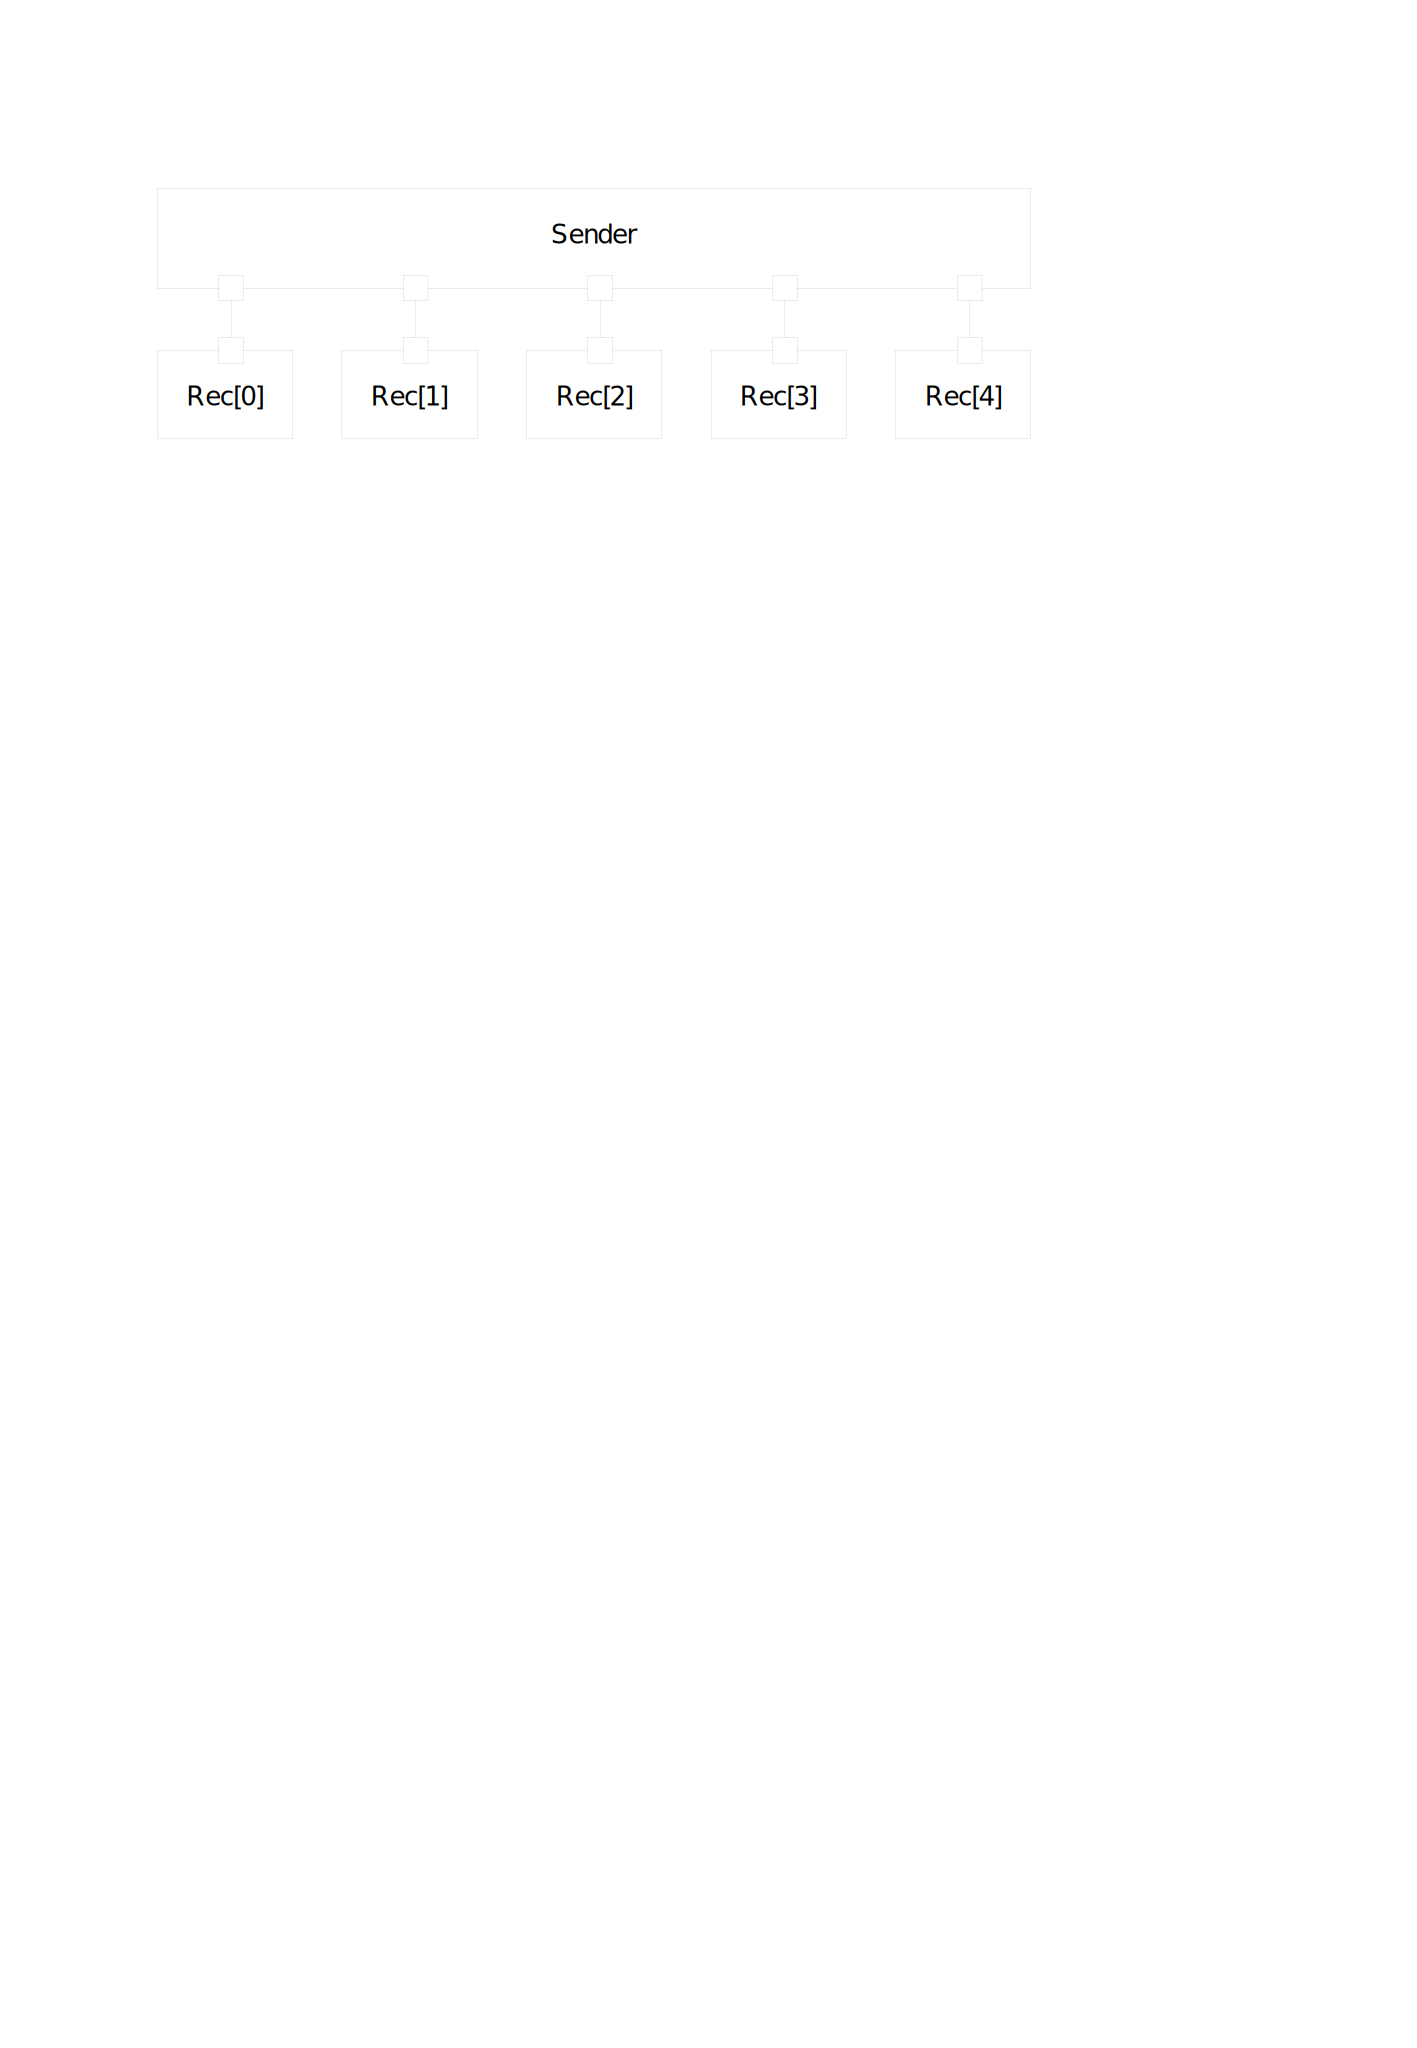
\includegraphics[width=4.625in, height=1.297in]{figures/usmanFig7}
\caption{Loop connection}
\label{fig:ch-ned-lang:loop-connection}
\end{center}
\end{figure}


One can place several connections in the body of the
\fpar[ned!keywords!for]{for} statement, separated by semicolons.

More than one indices can be specified in a for statement, with their
own lower and upper bounds. This will be interpreted as nested for
statements\index{ned!nested for statements}, the leftmost index being
the outermost and the rightmost index being the innermost loop.


\begin{Verbatim}[commandchars=\\\{\}]
\tbf{for} i=0..4, j=0..4 \tbf{do}
    //...
\tbf{endfor}
\end{Verbatim}

One can also use an index in the lower and upper bound expressions 
of the subsequent indices:

\begin{Verbatim}[commandchars=\\\{\}]
\tbf{for} i=0..3, j=i+1..4 \tbf{do}
    //...
\tbf{endfor}
\end{Verbatim}


In the above example, the following \textit{(i,j)} pairs will be used 
for the connections inside the for statement:

\tab \textit{(0,1)\tab (0,2)\tab (0,3)\tab (0,4)\tab (1,2)\tab (1,3)\tab (1,4)\tab (2,3)\tab (2,4)\tab (3,4)}

A gate cannot be used in more than one connection and one connection 
cannot be made more than once. Consider the following bogus statement:


\begin{Verbatim}[commandchars=\\\{\}]
\tbf{for} i = 0..2, j = 0..2 \tbf{do}
    module1.out [i] --> module2.in [\tbf{\textit{i}}];
\tbf{endfor}
\end{Verbatim}


It will cause a runtime error: each connection is made twice, 
as the index variable \textit{j} is not used in the connection. In 
general, every connection inside a loop should use all the index 
variables at both sides of the connection.


\tbf{Conditional connections}

\index{connection!conditional}

Connections can be conditional. This is a conditional connection:

\index{ned!keywords!if}

\begin{Verbatim}[commandchars=\\\{\}]
\tbf{for} i=0..n \tbf{do}
    Sender.outgate[i] --\ttt{>} Receiver[i].ingate \tbf{if} i\%2==0;
\tbf{endfor}
\end{Verbatim}


This way we connected every second gate.


\tbf{The nocheck modifier}



Conditional connections are especially useful with random numbers when
they can create random connections\index{connection!random}. Here, a
problem can be that by default, the simulation program checks if all
gates are connected. You can turn off this check by using the
\fpar[ned!keywords!nocheck]{nocheck} modifier
\index{gate!un-connected|see{ned keywords nocheck}}.

This example generates a random subgraph of a full graph:


\begin{Verbatim}[commandchars=\\\{\}]
\tbf{module} Stochastic:
    \tbf{parameters}: //..
    \tbf{gates}: //..
    \tbf{submodules}: //..
    \tbf{connections} \tbf{nocheck}:
        \tbf{for} i=0..9 \tbf{do}
            Sender.outgate[i] --> Receiver[i].ingate
                                \tbf{if} uniform(0,1)<0.3;
        \tbf{endfor}
\tbf{endmodule}
\end{Verbatim}


When using \fpar[ned!keywords!nocheck]{nocheck}, it is the simple modules' responsibility 
not to send messages on gates that are not connected.





\section{Parameterized compound modules}

\index{module!compound}

With the help of conditional parameter and gatesize blocks and 
conditional connections\index{connection!conditional}, one can create complex topologies.





\subsection{Examples}

\tbf{Example 1: Router}

The following example contains a router module with the number of
ports taken as parameter. The compound module is built using three
module types: Application, RoutingModule, DataLink. We assume that
their definition is in a separate NED file which we will import.


\begin{Verbatim}[commandchars=\\\{\}]
\tbf{import} "modules";
\tbf{module} Router:
    \tbf{parameters}:
        rte_processing_delay, rte\_buffersize,
        num_of_ports: \tbf{const};
    \tbf{gates}:
        \tbf{in}: input_ports[];
        \tbf{out}: output_ports[];
    \tbf{submodules}:
        local_user: Application;
        routing: RoutingModule
            \tbf{parameters}:
                processing_delay = rte_processing_delay,
                buffersize = rte_buffersize;
            \tbf{gatesizes}:
                input[num_of_ports+1],
                output[num_of_ports+1];
        port_if: DataLink[num_of_ports]
            \tbf{parameters}:
                retry_count = 5,
                window_size = 2;
    \tbf{connections}:
        \tbf{for} i=0..num_of_ports-1 \tbf{do}
            routing.output[i] --> port\_if[i].from_higher_layer;
            routing.input[i] <-- port_if[i].to_higher_layer;
            port_if[i].to_port --> output_ports[i];
            port_if[i].from_port <-- input_ports[i];
        \tbf{endfor;}
        routing.output[num_of_ports] --> local_user.input;
        routing.input[num_of_ports] <-- local_user.output;
\tbf{endmodule}
\end{Verbatim}


\tbf{Example 2: Chain}


For example, one can create a chain\index{chain} of modules like this:


\begin{Verbatim}[commandchars=\\\{\}]
\tbf{module} Serial:
    \tbf{parameters}: count: \tbf{const};
    \tbf{submodules}:
        node : Node [count]
            \tbf{gatesizes}:
                in[2], out[2];
            \tbf{gatesizes} \tbf{if} index==0 || index==count-1:
                in[1], out[1];
    \tbf{connections}:
        \tbf{for} i = 0..count-2 \tbf{do}
            node[i].out[i!=0 ? 1 : 0] --> node[i+1].in[0];
            node[i].in[i!=0 ? 1 : 0] <-- node[i+1].out[0];
        \tbf{endfor}
\tbf{endmodule}
\end{Verbatim}


\tbf{Example 3: Binary Tree}


Building a binary tree\index{binary tree} is a good example of using conditional 
connections:


\begin{Verbatim}[commandchars=\\\{\}]
\tbf{simple} BinaryTreeNode: 
    \tbf{gates}: 
        \tbf{in}: from_up, from_downleft, from_downright; 
        \tbf{out}: upward, downleft, downright;
\tbf{endsimple}

\tbf{module} BinaryTree:
    \tbf{parameters}: height: \tbf{const}; 
    \tbf{submodules}: node: BinaryTreeNode [ 2^height-1 ]; 
        //....
    \tbf{connections}:
        \tbf{for} i = 0..2^height-2, j = 0..2^height-2 \tbf{do} 
            node[i].upward --> node[j].from_downleft \tbf{if} leftchild(i,j); 
            node[i].from_up <-- node[j].downleft \tbf{if} leftchild(i,j); 
            node[i].upward --> node[j].from_downright \tbf{if} rightchild(i,j); 
            node[i].from_up <-- node[j].downright \tbf{if} rightchild(i,j); 
        \tbf{endfor} 
        //....
\tbf{endmodule}
\end{Verbatim}



The dotted lines should be replaced by modules that close the tree at
its root and the lower edge. The $leftchild(i,j)$ and
$rightchild(i,j)$ functions are:

\begin{eqnarray*}
leftchild(i,j)  & = & \left\{
    \begin{array}{r@{\quad:\quad}l}
      1 & i=2j+1\\
      0 & \mbox{otherwise}
    \end{array}
    \right.\\
rightchild(i,j) & = & \left\{
    \begin{array}{r@{\quad:\quad}l}
      1 & i=2j+2\\
      0 & \mbox{otherwise}
    \end{array}
    \right.
\end{eqnarray*}

These formulas can be directly substituted in the NED description, 
or alternatively, written in C and linked into the simulation 
executable.


\tbf{Example 4: Random graph}

Conditional connections can also be used to generate random
topologies\index{topology!random}.  The following code generates a
random subgraph of a full graph:


\begin{Verbatim}[commandchars=\\\{\}]
\tbf{module} RandomGraph:
    \tbf{parameters}:
        count: \tbf{const},
        connectedness; // 0.0<x<1.0
    \tbf{submodules}:
        node: Node [count]
            \tbf{gatesizes}: \tbf{in}[count], \tbf{out}[count];
    \tbf{connections} \tbf{nocheck}:
        \tbf{for} i=0..count-1, j=0..count-1 \tbf{do}
            node[i].out[j] --> node[j].in[i]
                \tbf{if} i!=j and uniform(0,1)<connectedness;
        \tbf{endfor}
\tbf{endmodule}
\end{Verbatim}


Note that not each gate of the modules will be connected. By default,
an unconnected gate produces a run-time error message when the
simulation is started, but this error message is turned off here with
the \fpar[ned!keywords!nocheck]{nocheck} modifier.  Consequently, it
is the simple modules' responsibility not to send on a gate which is
not leading anywhere.





\subsection{Using const with parameterized topologies}


Since parameter values can be used in defining the internal topology
of the module, the \fpar[ned!keywords!const]{const} modifier has a
significant role. Consider the following example:


\begin{Verbatim}[commandchars=\\\{\}]
\tbf{simple} Sender
    \tbf{parameters}:
        num_of_outgates;
    \tbf{gates}:
        \tbf{out}: outgate[num_of_outgates];
\tbf{endsimple} Sender

\tbf{simple} Receiver
    \tbf{gates}:
        \tbf{in}: ingate;
\tbf{endsimple} Receiver

\tbf{module} Network;
    \tbf{parameters}:
        num_of_mods: \tbf{const};
    \tbf{submodules}:
        sender: Sender
            \tbf{parameters}:
                num_of_outgates = \textit{num_of_mods};
        receiver: Receiver [\textit{num_of_mods}]
    \tbf{connections}:
        \tbf{for} i=1..\textit{num_of_mods} \tbf{do}
            sender.outgate[i] --> receiver[i].ingate
        \tbf{endfor};
\tbf{endmodule}

\tbf{network} net: Network
    \tbf{parameters}:
        num_of_mods = normal (5,2);
\tbf{endnetwork}
\end{Verbatim}


If parameter num\_of\_mods wasn't const, the following would happen:\\
normal(5,2) would be substituted for the num\_of\_mods. There 
are three places where an evaluation of num\_of\_mods (that is, normal 
(5,2)) is done (they are typed in italics in the example). It 
is likely that these evaluations would not result in the same 
value, and consequently, the gate vector sizes would not match 
each other and the end value of the for statement. Thus, the 
loop connection would not be created properly.

Using \fpar[ned!keywords!const]{const} for the parameter num\_of\_mods
prevents this from happening: an evaluation of normal(5,2) is
substituted for num\_of\_mods and an equal number of gates are
created.





\subsection{Design patterns for compound modules}

\index{module!compound!patterns}
\index{topology!patterns}

Several approaches can be used when you want to create complex 
topologies which have a regular structure; three of them are 
described below. 


\tbf{'Subgraph of a Full Graph' }


This pattern takes a subset of the connections of a full graph.  A
condition is used to ''carve out'' the necessary interconnection from
the full graph:


\begin{Verbatim}[commandchars=\\\{\}]
for i=0..N-1, j=0..N-1 do 
    node[i].out[...] --> node[j].in[...] if condition(i,j);
endfor
\end{Verbatim}




The RandomGraph compound module (presented earlier) is an example of
this pattern, but the pattern can generate any graph where an
appropriate \textit{condition(i,j)} can be formulated. For example,
when generating a tree\index{topology!tree} structure, the condition
would return whether node \textit{j} is a child of node \textit{i} or
vica versa.

Though this pattern is very general, its usage can be prohibitive if
the \textit{N} number of nodes is high and the graph is sparse (it has
much fewer connections that \textit{N}$^{\mathit{2}}$). The following
two patterns do not suffer from this drawback.


\tbf{'Connections of Each Node' }


The pattern loops through all nodes and creates the necessary
connections for each one. It can be generalized like this:


\begin{Verbatim}[commandchars=\\\{\}]
for i=0..Nnodes, j=0..Nconns(i)-1 do 
    node[i].out[j] --> node[rightNodeIndex(i,j)].in[j];
endfor
\end{Verbatim}



The Hypercube\index{topology!hypercube} compound module (to be
presented later) is a clear example of this approach. BinaryTree can
also be regarded as an example of this pattern where the inner j loop
is unrolled.

The applicability of this pattern depends on how easily the \textit{rightNodeIndex(i,j)} 
function can be formulated. 


\tbf{'Enumerate All Connections' }


A third pattern is to list all connections within a loop: 


\begin{Verbatim}[commandchars=\\\{\}]
for i=0..Nconnections-1 do 
    node[leftNodeIndex(i)].out[...] --> node[rightNodeIndex(i)].in[...];
endfor
\end{Verbatim}



The pattern can be used if \textit{leftNodeIndex(i)} and \textit{rightNodeIndex(i)} 
mapping functions can be sufficiently formulated.

The Serial module is an example of this approach where the mapping 
functions are extremely simple: \textit{leftNodeIndex(i)=i} and \textit{rightNodeIndex(i)=i+1}. 
The pattern can also be used to create a random subset of a full 
graph with a fixed number of connections.

In the case of irregular structures where none of the above patterns 
can be employed, the user can resort to specifying constant submodule/gate 
vector sizes and explicitly listing all connections, like he/she 
would do it in most existing simulators.





\subsection{Topology templates}
\label{sec:ch-ned-lang:topology-templates}



\tbf{Overview}


Topology templates are nothing more than compound modules where one or
more submodule types are left as parameters (using the
\fpar[ned!keywords!like]{like} phrase of the NED language).  You can
write such modules which implement mesh\index{topology!mesh},
hypercube\index{topology!hypercube},
butterfly\index{topology!butterfly}, perfect
shuffle\index{topology!perfect shuffle} or other topologies, and you
can use them wherever needed in you simulations.  With topology
templates\index{topology!templates}, you can reuse
\textit{interconnection structure}.



\tbf{An example: hypercube}


The concept is demonstrated on a network with hypercube interconnection. 
When building an N-dimension hypercube, we can exploit the fact 
that each node is connected to N others which differ from it 
only in one bit of the binary representations of the node indices 
(see Fig. \ref{fig:ch-ned-lang:hypercube-topology}). 

\begin{figure}[htbp]
  \begin{center}
    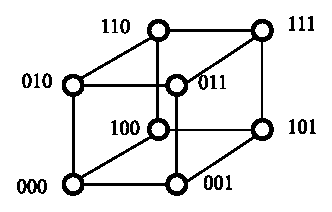
\includegraphics[width=2.111in, height=1.285in]{figures/usmanFig8}
    \caption{Hypercube topology}
    \label{fig:ch-ned-lang:hypercube-topology}
  \end{center}
\end{figure}


The hypercube topology\index{topology!hypercube} template is the
following (it can be placed into a separate file, e.g hypercube.ned):


\begin{Verbatim}[commandchars=\\\{\}]
simple Node 
    gates: out: out[]; in: in[];
endsimple

\tbf{module Hypercube}
    parameters:
        dim, nodetype; 
    submodules:
        node: nodetype[2{\textasciicircum}dim] like Node
    gatesizes:
        out[dim], in[dim];
    connections:
        for i=0..2^dim-1, j=0..dim-1 do
            node[i].out[j] --> node[i # 2^j].in[j]; // # is bitwise XOR 
        endfor
endmodule
\end{Verbatim}



When you create an actual hypercube, you substitute the name 
of an existing module type (e.g. Hypercube\_PE) for the nodetype 
parameter. The module type implements the algorithm the user 
wants to simulate and it must have the same gates that the Node 
type has. The topology template code can be used through importing 
the file: 


\begin{Verbatim}[commandchars=\\\{\}]
import "hypercube.ned"
  
simple Hypercube_PE
    gates: out: out[]; in: in[];
endsimple

network hypercube: Hypercube 
    parameters:
        dim = 4,
        nodetype = "Hypercube_PE";
endnetwork
\end{Verbatim}



If you put the nodetype parameter to the ini file, you can use the
same simulation model to test e.g. several routing algorithms in a
hypercube, each algorithm implemented with a different
simple module type -- you just have to supply
different values to nodetype, such as ''WormholeRoutingNode'',
''DeflectionRoutingNode'', etc.





\section{Network definition}

\index{ned!network definition}

A \textit{network} \textit{definition} (or \textit{system module
  definition}) specifies the system module. In its syntax, it is very
similar to a submodule declaration. The system definition starts with
keyword \fpar[ned!keywords!network]{network} and ends with
\fpar[ned!keywords!endnetwork]{endnetwork}.


An example:


\begin{Verbatim}[commandchars=\\\{\}]
\tbf{network} modelledNetwork: SomeModule
    \tbf{parameters}:
        par1=10,
        par2=normal(100,20);
\tbf{endnetwork}
\end{Verbatim}


Here, SomeModule is the name of a compound or a simple module type.


There can be several system definitions in a network description, 
each one defines a different network. The simulation program 
built with such a network description is able to run any of them; 
the desired one can be specified in the config file (see later).





\section{Support for parallel execution}

\opp simulations can be executed in parallel\index{parallel
  simulation}. This means that different parts of the model execute on
different hosts or processors.  (We'll use the term ''host'' or
''machine'' in this sense.) The unit of granularity is the
simple module: one simple
module always executes on a single processor.


Parallel execution is also supported by NED: the language provides 
an elegant way of specifying execution hosts for different modules. 
We'll discuss this feature in the following sections.





\subsection{Extensions to the compound module and system definitions}

To support the segmentation\index{segmentation} of the model for
execution of different modules, the compound module definition was
extended with the \fpar[ned!keywords!machines]{machines:} and the \fpar[ned!keywords!on]{on:} keywords.

Example:
\begin{Verbatim}[commandchars=\\\{\}]
\tbf{module} SomeNameForCompoundModule
    \tbf{machines}: host1, host2, host3, host4;
    \tbf{parameters}: //...
    \tbf{gates}: //...
    \tbf{submodules}: 
        submodule1 : submodtype1
            \tbf{on:} host1;
        submodule2 : submodtype2
            \tbf{on:} host2, host3;
        submodule3 : submodtype1
            \tbf{on:} host4;
    \tbf{connections}: //...
\tbf{endmodule}
\end{Verbatim}


The \fpar[ned!keywords!machines]{machines:} section lists formal host
names which are used in the \fpar[ned!keywords!on]{on:} lists of the
submodules.


In the example, the second submodule is itself a compound module that
can be further subdivided to run on two separate hosts, so its
definition must have a machines: section with two parameters.  You do
not have to propagate host names down to simple module level: you can
stop at a compound module which executes on a single host. In other
words, a compound module with no machines: section is equivalent to
one with one machine parameter.

Of course, you can give the same value to several machine parameters,
as to submodule1's in the following example. In this case, the whole
compound module will be placed on a single host, as if it never had
machine parameters at all.


\begin{Verbatim}[commandchars=\\\{\}]
\tbf{module} AnotherCompoundModule
    \tbf{machines}: host1, host2;
    \tbf{parameters}: //...
    \tbf{gates}: //...
    \tbf{submodules}: 
        submodule1 : submodtype1
            \tbf{on:} host1, host1, host1;
        //...
    \tbf{connections}: //...
\tbf{endmodule}
\end{Verbatim}


Host names propagate up to network definition level. Extension 
to the network definition:


\begin{Verbatim}[commandchars=\\\{\}]
\tbf{network} distVector: DistVector
    on: machine1, machine2, machine3;
\tbf{endnetwork}
\end{Verbatim}



The \fpar[ned!keywords!on]{on:} parameters of the network definition
can be actual host names, or alternatively, they can be symbolic names
that are mapped to actual host names in the config file.





\subsection{Conditional 'on' sections}

Similarly to the parameters: and gatesizes: section, multiple
\fpar[ned!keywords!on]{on:} sections can exist for the submodules if
they are tagged with \fpar[ned!keywords!if]{if} phrases.

This makes it possible to control the module distribution with
parameters. You can even put different parts of a module vector on
different machines using the index operator\index{index operator} (see
later in Section \ref{ch-ned-lang:sec:expressions}, Expressions).

Example:


\begin{Verbatim}[commandchars=\\\{\}]
\tbf{module} DistVector:
    \tbf{machines}: host1, host2, host3;
    \tbf{submodules}:
        node : Node [count]
            \tbf{on} \tbf{if} index<count*.33: host1;
            \tbf{on} \tbf{if} index>=count*.33 && index<count*.66: host2;
            \tbf{on} \tbf{if} index>=count*.66: host3;
\tbf{endmodule}
\tbf{network} distvector: DistVector
    on machine1, machine2, machine3;
\tbf{endnetwork}
\end{Verbatim}






\section{Expressions}
\label{ch-ned-lang:sec:expressions}

In the NED language there are a number of places where
expressions\index{ned!expressions} are expected.


When such an expression is encountered by the NEDC compiler, it is
compiled and it will be evaluated\index{ned!expressions!evaluation}
run-time.

Expressions have a C-style syntax. They are built with the usual math
operators\index{math operators}; they can use parameters taken by
value or by reference; call C functions; contain random and input
values etc.





\subsection{Using parameters in expressions (ref and ancestor)}

Expressions can use the parameters of the compound module being built.
A parameter can be taken by value\index{ned!parameters!by value} or by
reference\index{ned!parameters!by reference}. The default is by value;
to select by-reference passing for a parameter, you have to use the
\fpar[ned!keywords!ref]{ref} modifier. Parameters passed by
reference can be used by a module to propagate values (status info
etc.)  to other modules.

The ancestor modifier allows one to access parameters from higher 
in the module hierarchy.


\begin{Verbatim}[commandchars=\\\{\}]
\tbf{module} Compound
    \tbf{parameter}: nnn;
    \tbf{submodules}:
        proc: Processor
            \tbf{parameters}:
                par1 = \tbf{ref} nnn / 2,
                par2 = 10 * \tbf{ancestor} par_somewhere_up;
\tbf{endmodule}
\end{Verbatim}





\subsection{Operators}

The following operators\index{ned!expressions!operators} can be used
in expressions, in order of precedence:


\begin{longtable}{|l|l|}
\hline
\tabheadcol
\tbf{Operator} & \tbf{Meaning}\\\hline
-, !, \ensuremath{\sim} & unary minus, negation, bitwise complement \\
{\textasciicircum}        & power of \\
 & \\
$*$, /, \%                & multiply, divide, modulus \\
 & \\
+, -                    & add, subtract \\
 & \\
\ttt{<}\ttt{<}, \ttt{>}\ttt{>}      & bitwise shifting \\
 & \\
\&, |, \#        & bitwise and, or, xor
                         \textit{({\textasciicircum} is reserved for power)} \\
 & \\
==                      & equal \\
!=                      & not equal \\
\ttt{>}, \ttt{>=}       & greater, greater or equal \\
\ttt{<}, \ttt{<=}       & less, less or equal \\
 & \\
\&\&, ||, \#\# & logical operators and, or, xor \\
 & \\
?:                      & the C/C++ ``inline if'' \\\hline
\end{longtable}






\subsection{The sizeof() and index operators}

A useful operator is sizeof()\index{ned!sizeof()}, which gives the
size of a vector gate\index{gate!vector}. The index
operator\index{ned!index operator} gives the index of the current
submodule in its module vector.

An example for both:

\begin{Verbatim}[commandchars=\\\{\}]
\tbf{module} Compound
    \tbf{gates}: \tbf{in}: fromgens[];
    \tbf{submodules}:
        proc: Processor[ \tbf{sizeof}(fromgens) ];
            \tbf{parameters}: address = 10*(1+\tbf{index});
    \tbf{connections}:
        \tbf{for} i = 0.. \tbf{sizeof}(fromgens)-1 \tbf{do}
            in[i] --> proc[i].input;
        \tbf{endfor}
\tbf{endmodule}
\end{Verbatim}


Here, we create as many processors as there are input gates for 
this compound module in the network. The address parameters of 
the processors are 10, 20, 30 etc.





\subsection{Time constants}

Anywhere you would put numeric constants\index{numeric constants}
(integer or real) to mean time in seconds, you can also specify the
time in units like milliseconds, minutes or hours:


\begin{Verbatim}[commandchars=\\\{\}]
    ... 
    \tbf{parameters}:
        propagation_delay = 560ms, // 0.560s
        connection\_timeout = 6m 30s 500ms, // 390.5s
        lunchtime = 0.5h; // 30 min
\end{Verbatim}


The following units\index{time units} can be used:

\begin{longtable}{|c|l|l|}
\hline
ns & nanoseconds & $*10^{-9}$ \\\hline
us & microseconds & $*10^{-6}$ \\\hline
ms & milliseconds & $*10^{-3}$ \\\hline
s  & seconds & $*1$ \\\hline
m  & minutes & $*60$ \\\hline
h  & hours & $*3600$ \\\hline
d  & days & $*60*3600$ \\\hline
\end{longtable}







\subsection{Random values}

{\opp} has the following predefined distributions\index{distribution!predefined}:
\begin{itemize}
  \item{uniform\index{distribution!uniform}, uniform integer}
  \item{exponential\index{distribution!exponential}}
  \item{normal\index{distribution!normal}, truncated normal\index{distribution!truncated normal}}
\end{itemize}

Each distribution has one or more parameters.

Examples:

\begin{Verbatim}
uniform(0,1)       // uniform in [0,1)
intuniform(-2,2)   // uniform int, limits included: -2,-1,0,1,or 2
exponential(5)     // exponential with mean=5 (thus parameter=0.2)
normal(100,5)      // mean 100, variance 5
truncnormal(5,3)   // normal distr, truncated to nonnegative values
\end{Verbatim}

The functions all use the random number generator 0. By using the
genk\_-prefixed\index{distribution!genk\_-prefixed} versions of the
above functions, you can specify which generator should be used. The
index of the generator comes as the first argument.


Example:

\begin{Verbatim}
genk_normal(2,100,5) // as normal(100,5), using generator 2
\end{Verbatim}


The above distributions are implemented with C functions (see later in
the Functions section). This also means that you can easily add
further ones by writing their code in C++ and using the
\fmac{Register\_Function()} macro. Your distributions will be treated
in the same way as the built-in ones.





\subsection{Input value}

The syntax is:


\begin{Verbatim}[commandchars=\\\{\}]
    \tbf{input}( 10, "Number of processors:" )
\end{Verbatim}


Or you can omit the prompt text:

\begin{Verbatim}[commandchars=\\\{\}]
    \tbf{input}( 10ms )
\end{Verbatim}


Value for input parameters\index{input parameters} can be given in the
config file. If they are not there, the user will be offered a prompt
to enter the value.





\subsection{Functions}
\index{ned!functions}

In NED expressions, you can use mathematical functions:
\begin{itemize}
  \item{many of the C language's \ttt{<math.h>} library functions:
    \ttt{exp()}, \ttt{log()}, \ttt{sin()}, \ttt{cos()}, \ttt{floor()},
    \ttt{ceil()}, \ttt{etc.}}
  \item{functions that generate random variables: \ttt{uniform},
    \ttt{exponential}, \ttt{normal} and others were already
    discussed.}
  \item{user defined functions that can implement new functions or
    yield random variables of distributions that are originally not
    built in.}
\end{itemize}


To use user-defined functions\index{functions!user-defined}, one has
to code the function in C++.  The C++ function must take 0, 1, 2, or 3
arguments of type double and return a double. The function must be
registered in one of the C++ files with the \fmac{Define\_Function()}
macro.

An example function (the following code must appear in one of the C++
sources):


\begin{Verbatim}
#include <omnetpp.h>

double average(double a, double b)
{
  return (a+b)/2;
}

Define_Function(average, 2);
\end{Verbatim}


The number 2 means that the \fname{average()} function has 2
arguments.  After this, the \fname{average()} function can be used in
NED files:


\begin{Verbatim}[commandchars=\\\{\}]
\tbf{module} Compound
    \tbf{parameter}: a,b;
    \tbf{submodules}:
        proc: Processor
            \tbf{parameters}: av = average(a,b);
\tbf{endmodule}
\end{Verbatim}


An important application of this concept is to extend {\opp} 
with new distributions.





\subsection{Display strings}
\label{sec:ch-ned-lang:display-strings}

Display strings\index{display strings} specify the arrangement and
appearance of modules in graphical user interfaces (currently only
Tkenv): they control how the objects (compound modules, their
submodules and connections) are displayed. Display strings occur in
NED description's \fpar[ned!keywords!display]{display:}
phrases.

The display string format is a semicolon-separated list of tags. 
Each tag consists of a key (usually one letter), an equal sign 
and a comma-separated list of parameters, like:

\begin{Verbatim}
  "p=100,100;b=60,10,rect;o=blue,black,2"
\end{Verbatim}  

Parameters may be omitted also at the end and also inside the 
parameter list, like:

\begin{Verbatim}
  "p=100,100;b=,,rect;o=blue,black"
\end{Verbatim}

Module/submodule parameters can be included with the \ttt{\$name} notation:

\begin{Verbatim}
  "p=$xpos,$ypos;b=rect,60,10;o=$fillcolor,black,2"
\end{Verbatim}
%%$

Objects that may have display strings are:
\begin{itemize}
  \item{compound modules (as the enclosing module in the drawing),}
  \item{submodules}
  \item{connections}
\end{itemize}

\tbf{Tags used in submodule display strings:}

\index{display strings!tags}

\begin{longtable}{|p{6cm}|p{8cm}|}
\hline
% ROW 1
\tabheadcol
\tbf{Tag} & \tbf{Meaning} \\\hline
% ROW 2
\tbf{p=}\textit{xpos},\textit{ypos}
&
{\raggedright Place submodule at (\textit{xpos},\textit{ypos}) pixel position, with the origin being the top-left corner of the enclosing module.\\
 Defaults: an appropriate automatic layout is where submodules 
do not overlap.\\
If applied to a submodule vector, \textit{ring} or \textit{row} layout is 
selected automatically.}\\\hline
% ROW 3
\tbf{p=}\textit{xpos},\textit{ypos},\tbf{row},\textit{deltax} &
{\raggedright Used for module vectors. Arranges submodules in a row starting 
at (\textit{xpos},\textit{ypos}), keeping \textit{deltax} distances. \\
Defaults: \textit{deltax} is chosen so that submodules do not overlap. \\
\tbf{row} may be abbreviated as \tbf{r}.}\\\hline
% ROW 4
\tbf{p=}\textit{xpos},\textit{ypos},\tbf{column},\textit{deltay}
&
{\raggedright Used for module vectors. Arranges submodules in a column starting 
at (\textit{xpos},\textit{ypos}), keeping \textit{deltay} distances. \\
Defaults: \textit{deltay} is chosen so that submodules do not overlap. \\
\tbf{column} may be abbreviated as \tbf{col} or \tbf{c}.}\\\hline
% ROW 5
\tbf{p=}\textit{xpos},\textit{ypos},\tbf{matrix},
\textit{itemsperrow},\textit{deltax},\textit{deltay}
& 
{\raggedright Used for module vectors. Arranges submodules in a matrix starting 
at (\textit{xpos},\textit{ypos}), at most \textit{itemsperrow} submodules in 
a row, keeping \textit{deltax} and \textit{deltay} distances. \\
Defaults: \textit{itemsperrow}=5, \textit{deltax,deltay} are chosen so that 
submodules do not overlap. \\
\tbf{matrix} may be abbreviated as \tbf{m}.}\\\hline
% ROW 6
\tbf{p=}\textit{xpos},\textit{ypos},\tbf{ring},\textit{width,height}
& 
{\raggedright Used for module vectors. Arranges submodules in an ellipse, 
with the top-left corner of its bounding boxes at (\textit{xpos},\textit{ypos}), 
with the \textit{width} and \textit{height}. \\
Defaults: \textit{width}=40, \textit{height}=24 \\
\tbf{ring} may be abbreviated as \tbf{ri}.}\\\hline
% ROW 7
\tbf{p=}\textit{xpos},\textit{ypos},\tbf{exact},\textit{deltax},\textit{deltay}
& 
{\raggedright Used for module vectors. Each submodule is placed at \textit{(xpos+deltax}, \textit{ypos+deltay)}. 
This is useful if \textit{deltax} and \textit{deltay} are parameters (e.g.:\textit{''p=100,100,exact,\$x,\$y''}) 
which take different values for each module in the vector. \\
Defaults: \textit{none} \\
\tbf{exact} may be abbreviated as \tbf{e} or \tbf{x}.}\\\hline
% ROW 8
\tbf{b=}\textit{width},\textit{height},\tbf{rect}
& 
{\raggedright Rectangle with the given \textit{height} and \textit{width}.\\
Defaults: \textit{width}=40, \textit{height}=24}\\\hline
% ROW 9
\tbf{b=}\textit{width},\textit{height},\tbf{oval}
& 
{\raggedright Ellipse with the given \textit{height} and \textit{width}.\\
Defaults: \textit{width}=40, \textit{height}=24}\\\hline
% ROW 10
\tbf{o=}\textit{fillcolor},\textit{outlinecolor},\textit{borderwidth}
& 
{\raggedright Specifies options for the rectangle or oval. Any valid Tk color 
specification is accepted: English color names or \textit{\#rgb}, \textit{\#rrggbb} 
format (where \textit{r},\textit{g},\textit{b} are hex digits). \\
Defaults: \textit{fillcolor}=\#8080ff (a lightblue), \textit{outlinecolor}=black, \textit{borderwidth}=2}\\\hline
% ROW 11
\tbf{i=}\textit{iconname}
&
{\raggedright Use the named icon. \\
No default. If no icon name is present, \textit{box} is used.}\\\hline
\end{longtable}



Examples:

\begin{Verbatim}
  "p=100,60;i=workstation"
  "p=100,60;b=30,30,rect;o=4"
\end{Verbatim}


\tbf{Tags used in enclosing module display strings:}


\begin{longtable}{|p{6cm}|p{8cm}|}
\hline
% ROW 1
\tabheadcol
\tbf{Tag} & \tbf{Meaning}\\
\hline
% ROW 2
\tbf{p=}\textit{xpos},\textit{ypos} & Place enclosing module at (\textit{xpos},\textit{ypos}) pixel position, with (0,0) being the top-left corner of the window.\\
\hline
% ROW 3
\tbf{b=}\textit{width},\textit{height},\tbf{rect}
& 
{\raggedright Display enclosing module as a rectangle with the given \textit{height} 
and \textit{width}.\\
Defaults: \textit{width,} \textit{height} are chosen automatically}\\\hline
% ROW 4
\tbf{b=}\textit{width},\textit{height},\tbf{oval}
& 
{\raggedright Display enclosing module as an ellipse with the given \textit{height} 
and \textit{width}.\\
Defaults: \textit{width,} \textit{height} are chosen automatically}\\\hline
% ROW 5
\tbf{o=}\textit{fillcolor},\textit{outlinecolor},\textit{borderwidth}
& 
{\raggedright Specifies options for the rectangle or oval. Any valid Tk color 
specification is accepted: English color names or \textit{\#rgb}, \textit{\#rrggbb} 
format (where \textit{r},\textit{g},\textit{b} are hex digits).\\
Defaults: \textit{fillcolor}=\#8080ff (a lightblue), \textit{outlinecolor}=black, \textit{borderwidth}=2}\\\hline
\end{longtable}



\tbf{Tags used in connection display strings:}

\begin{longtable}{|p{6cm}|p{8cm}|}
\hline
% ROW 1
\tabheadcol
\tbf{Tag} & \tbf{Meaning}\\
\hline
% ROW 2
{\raggedright \tbf{m=auto}\\
\tbf{m=north}\\
\tbf{m=west}\\
\tbf{m=east}\\
\tbf{m=south}}
& 
Drawing mode. Specifies the exact placement of the connection 
arrow. The arguments can be abbreviated as a,e,w,n,s.\\\hline
% ROW 3
{\raggedright \tbf{m=manual},\textit{srcpx},\textit{srcpy},\\
  \textit{destpx},\textit{destpy}}
& 
{\raggedright The manual mode takes four parameters that explicitly specify 
anchoring of the ends of the arrow: \textit{srcpx}, \textit{srcpy}, \textit{destpx}, \textit{destpy}. 
Each value is a percentage of the width/height of the source/destination 
module's enclosing rectangle, with the upper-left corner being 
the origin. Thus,
\begin{Verbatim}
m=m,50,50,50,50
\end{Verbatim}
would connect the centers of the two module rectangles.}\\\hline
% ROW 4
\tbf{o=}\textit{color},\textit{width} & 
Specifies the appearance of the arrow. Any valid Tk color specification 
is accepted: English color names or \#rgb, \#rrggbb specification 
(where r,g,b are hex digits). \linebreak
Defaults: \textit{color}=black, \textit{width}=2\\
\hline
\end{longtable}



Examples:
\begin{Verbatim}
  "m=a;o=blue,3"
\end{Verbatim}





\section{GNED -- Graphical NED Editor}

\index{ned!graphical interface}

The GNED editor allows you to design compound modules graphically.
GNED works with NED files -- it doesn't use any nasty internal file
format. You can load any of your existing NED files, edit the compound
modules in it graphically and then save the file back. The rest of the
stuff in the NED file (simple modules, channels, networks etc.) will
survive the operation. GNED puts all graphics-related data into
display strings.


GNED works by parsing your NED file into an internal data structure, 
and regenerating the NED text when you save the file. One consequence 
of this is that indentation will be ''canonized'' 
-- hopefully you consider this fact as a plus and not as a minus. 
Comments in the original NED are preserved -- the parser associates 
them with the NED elements they belong to, so comments won't 
be messed up even if you edit the graphical representation to 
death by removing/adding submodules, gates, parameters, connections, 
etc.

GNED is now a fully two-way visual tool. While editing the graphics, 
you can always switch to NED source view, edit in there and switch 
back to graphics. Your changes in the NED source will be immediately 
backparsed to graphics; in fact, the graphics will be totally 
reconstructed from the NED source and the display strings in 
it.

GNED is still under development. There are some missing functions 
and bugs, but overall it should be fairly reliable. See the TODO 
file in the GNED source directory for problems and missing features.


\tbf{Comment parsing:}


It is useful to know how exactly GNED identifies the comments 
in the NED file. The following (maybe a bit long) NED code should 
explain it:

\begin{Verbatim}
// ---------------------------------------------------------------
// File: sample.ned
//
// This is a file comment. File comments reach from the top of 
// the file till the last blank line above the first code line.
// ---------------------------------------------------------------
//

// The file comment can also contain blank lines, so this is 
// still part of the above file comment.
//
// Module1 --
//
// This is a banner comment for the Module1 declaration below.
// Banner comments can be multi-line, but they are not supposed 
// to contain blank lines. (Otherwise the lines above the blank 
// one will be taken as part of a file comment or trailing comment.)
//
module Module1
    submodules: // and this is right-comment
// This is another banner comment, for the submodule
        submod1: Module;
            display: ''p=120,108;b=96,72,rect'';
            connections:
                out --> submod1.in; // Right-comments can also be
                                    // multi-line.
endmodule

// Finally, this is a trailing comment, belonging to the above
// module. It may contain blank lines. Trailing comments are 
// mostly used to put separator lines into the file, like this:
// --------------------------------------------------------------
// Module2 --
//
// an empty module
//
module Module2
endmodule
\end{Verbatim}


\tbf{Key/mouse bindings:}

\index{gned!mouse bindings}

In graphics view, there are two editing modes: draw and select/mode. 
The mouse bindings are the following:


\begin{longtable}{|p{7cm}|p{7cm}|}
\hline
% ROW 1
\tabheadcol
\tbf{Mouse} & \tbf{Effect}\\
\hline
% ROW 2
\multicolumn{2}{|c|}{\tbf{In} \tbf{\textit{draw}} \tbf{mode:}} \\
\hline
% ROW 3
Drag out a rectangle in empty area: &  create new submodule \\\hline
% ROW 4
Drag from one submodule to another: &  create new connection \\\hline
% ROW 5
Click in empty area: & switch to select/move mode \\\hline
% ROW 6
\multicolumn{2}{|c|}{\tbf{In} \tbf{\textit{select/move}} \tbf{mode:}} \\\hline
% ROW 7
Click submodule/connection: & select it\\\hline
% ROW 8
Ctrl-click submodule/conn.: & add to selection \\\hline
% ROW 9
Click in empty area: & clear selection\\\hline
% ROW 10
Drag a selected object: & move selected objects \\\hline
% ROW 11
Drag submodule or connection: & move it \\\hline
% ROW 12
Drag either end of connection: & move that end \\\hline
% ROW 13
Drag corner of (sub)module: & resize module\\\hline
% ROW 14
Drag starting in empty area: & select enclosed submodules/connections \\\hline
% ROW 15
\textit{Del} key & delete selected objects \\\hline
% ROW 16
\multicolumn{2}{|c|}{\tbf{Both editing modes:}} \\\hline
% ROW 17
Right-click on module/submodule/con\-nec\-tion: & popup menu \\\hline
% ROW 18
Double-click on submodule: & go into submodule \\\hline
% ROW 19
Click name label & edit name \\\hline
% ROW 20
Drag\&drop module type from the tree view to the canvas & 
create a submodule of that type \\\hline
\end{longtable}



%%% Local Variables: 
%%% mode: latex
%%% TeX-master: "usman"
%%% End: 
